
\chapter{Neural Network Framework}
\label{chapter:neural-network-learning}
Once the preprocessing stage is complete, and the source documents are ready for the main task, we feed them to a neural network for extraction of relational entities for GWAS population characteristics. We depend on Convolutional Neural Networks (CNNs) to detect the underlying semantic and syntactic relationship between these objects and extract the pairs from the new articles accordingly. This chapter describes the framework of our neural networks and their working to produce the final output. 

\section{Convolution Neural Networks}
\label{section:convolution-neural-networks}
In machine learning, a convolutional neural network (CNN) is a type of feed-forward artificial neural network which was primarily designed to overcome the problems associated with image processing while taking inspiration from neurobiology. Yann LeCunn et. al. tried to capture the organization of neurons in the visual cortex of the cat, which at that time was known to consist of maps of local receptive fields that decreased in granularity as the cortex moved anteriorly \cite{hubel1959receptive}. These neural networks utilize multiple layers of convolving filters that are applied to the local regions to recognize the underlying patterns in the input data. As opposed to multi-layer perceptron architecture, convolutional neural networks have certain distinguishing characteristics like local connectivity, replicated filters with shared weights structure and so on which allow these systems to achieve better generalization on vision problems. These features have made CNNs especially favorable for image and speech processing tasks.

The architecture of a convolutional neural network (CNN) is formed by stacking a multiple number of distinct layers which transform the input volume into an output result through a differentiable function. A typical CNN commonly uses a set of separate layers which perform individual operations and contribute to the overall function of transformation. The core building block of any CNN is the {\it convolution layer} where different filters convolve across the width and height of the input volume producing a feature map for that filter. A filter consists of a layer of connection weights, with the input being the size of a small 2-dimensional image patch and the output being a single unit. Since this filter is repeatedly applied, the resulting connectivity looks like a series of overlapping receptive fields which map to a matrix of the feature outputs. The network thus learns the filters that activate according to some particular feature in the input. 

Another important concept of CNNs is {\it pooling layer} which is a kind of non-linear down-sampling operation and provides a form of translation invariance. The function of the pooling layer is to progressively reduce the spatial size of the representation to reduce the total number of parameters and overall computation in the network which therefore also controls the amount of overfitting. Several non-linear functions exist which can be used to implement the pooling operation among which max pooling and average pooling are the most common. A typical CNN architecture may have multiple layers with alternating convolutional and pooling layers which eventually extracts most important features from the input image. By applying such a subsampling layer in between convolutional layers, we develop the spatial abstractness with the increasing feature abstractness. 

After several processing layers, the high-level reasoning in the neural network is done via {\it fully-connected layer} which has full connections to all the activations in the previous layer and culminates into a decision function in the form of a softmax or logistic operation. While training of the whole network takes quite some time, the convolutional neural network learns much faster than a standard feed-forward neural network and performs quite well in comparison to the previous neural network paradigms. A typical architecture of convolutional neural networks showing these layers is depicted in Figure \ref{figure:typical-cnn-architecture}

\begin{figure}[ht]
    \centering
    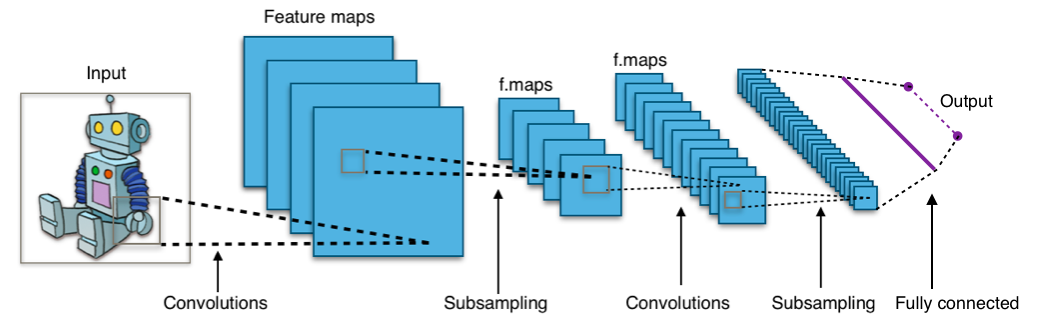
\includegraphics[width=0.85\linewidth]{Images/Typical-CNN-Architecture.png}
    \caption{A typical CNN architecture used for image processing showing multiple layers of convolutions function, each of which produces various feature maps, followed by subsampling layers with a final fully-connected layer.}
    \label{figure:typical-cnn-architecture}
    \vspace{0.2in}
\end{figure}

\section{Applications to Natural Language Processing}
\label{section:application-to-nlp}

Recently, convolutional neural networks have begun to overtake traditional sparse, linear models for natural language processing as they automatically learn the features from the sentences and minimize the dependence on external toolkits and resources. These models have been shown to be useful for various natural language processing problems and have achieved excellent results in semantic parsing \cite{grefenstette2014deep}, sentence modeling \cite{kalchbrenner2014convolutional}, sentence classification \cite{kim2014convolutional} and other traditional NLP tasks. Besides comprising different robust classifiers as part of their architecture, these neural networks are also used to train a neural language model which can generate sentences word by word \cite{son2012continuous}. Several models of convolutional neural networks have been applied to diverse content ranging from long-form texts (like movie reviews) to short texts (like tweets) and have shown good performance in each of these domains. 

The main difference in using these neural networks for natural language processing tasks from image processing functions concerns the input to these nets. We begin by converting a tokenized text snippet, of size $s$, to a matrix whose each row of is a word vector representation for a token in the text. These word vector representations might be outputs from trained {\it word2vec} \cite{mikolov2013distributed} or {\it GloVe} \cite{pennington2014glove} models with a fixed dimensionality, $d$, of the vectors. Another approach is to use one-hot vectors that index the word into a vocabulary and these vectors are updated accordingly while training the whole network \cite{johnson2014effective}. The various word embedding approaches can capture multiple different degrees of similarity between the words which can be used to reconstruct the linguistic contexts of these words. We can effectively treat the text matrix as an `image' of size $s \times d$ (with a predefined s) and perform convolutions on it through linear filters. 

As each row of this matrix represents a discrete token, the breadth of the convolving filters are identical to the dimensionality of the word vectors (i.e. $d$). Each filter slides over the original input matrix and for every position, we compute element-wise multiplication between the two matrices (the input text matrix and the filter matrix) and add the multiplications output to get the final integer which forms a single element of the `feature map'. It is important to note that a filter, of size $d \times h$, acts as feature detector from the original input by extracting features in a way similar to (but not limited to) multiple $h$-grams from the sentence and represent them in a more compact way using feature maps. These features maps are then sub-sampled to continue with a combination of the most important features. The final set of features is fed to a decision function using a fully connected layer to produce the final output as desired. Figure \ref{figure:cnn-textclassification-example} denotes a typical architecture of convolutional neural networks for sentence classification tasks \cite{collobert2011natural} which also forms the basis of our framework as discussed in next section. 

\begin{figure}[ht]
    \centering
    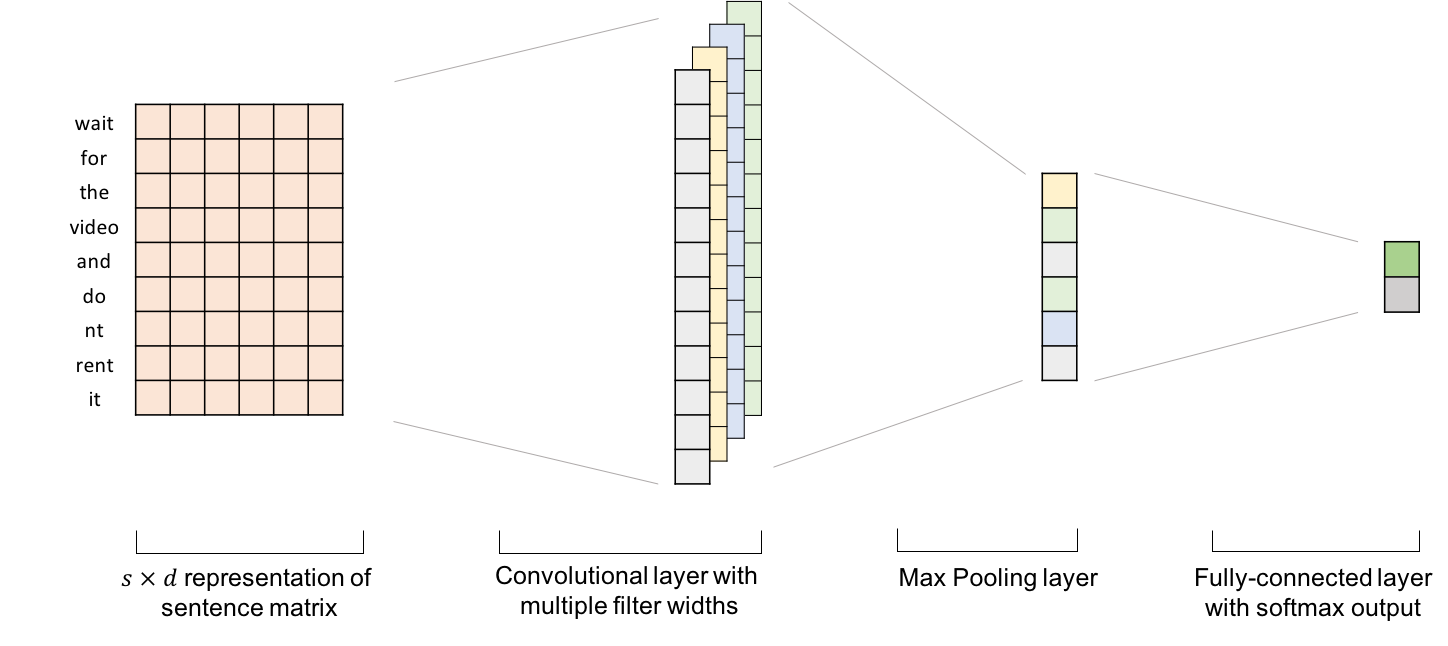
\includegraphics[width=0.85\linewidth]{Images/CNN-TextClassification-Example.png}
    \caption{Illustration of a Convolutional Neural Network (CNN) architecture for sentence classification with a fixed-size input vector matrix followed by a convolutional, a pooling, and a fully-connected layer.}
    \label{figure:cnn-textclassification-example}
\end{figure}

\section{Our Framework}
\label{section:our-framework}

As mentioned in the previous section, the architecture for our convolutional neural network for the task of relation extraction is based on an approach to sentence classification by Collobert et. al. \cite{collobert2011natural}. The model proposed by us takes as input the raw sentence snippets with annotated entity mentions and produces a final boolean output indicating if the tagged items do (or do not) exhibit the corresponding relationship between them. The input text comprising of varying-sized words are first transformed into fixed length vectors which are understandable to the network using word and position embeddings. These vectors are subsequently fed into a convolutional layer where multiple filters convolve over the input to extract various related features in the form of feature maps. These feature maps are pooled using a max function to create a feature vector of most important features in the input sentence. The logistic function finally uses this feature vector in the fully-connected layer to produce the final output as desired. The entire architecture of our convolutional neural network is depicted in Figure \ref{figure:basic-cnn-framework} while we discuss each layer in more details below. 

\afterpage{
    \begin{figure}[b]
        \centering
        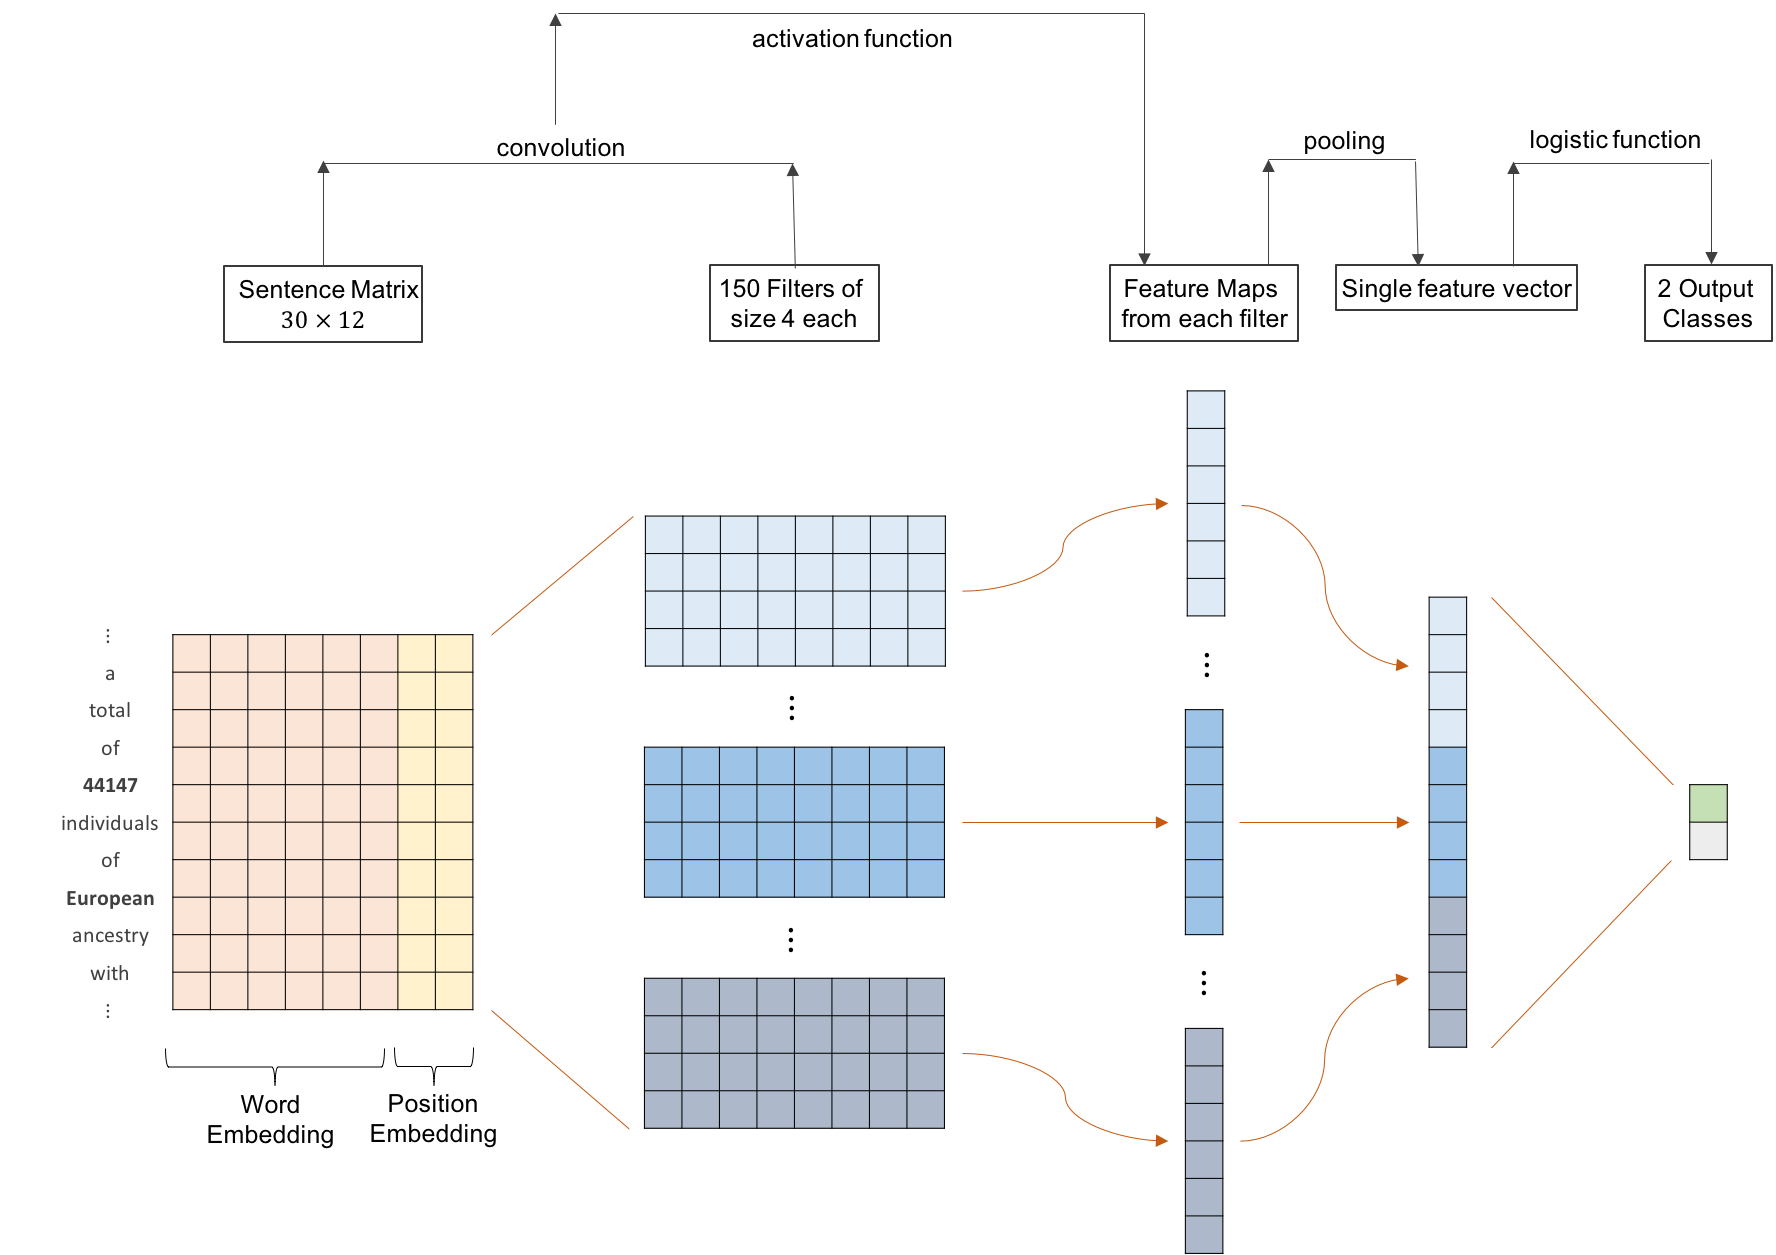
\includegraphics[width=\linewidth]{Images/CNN-Framework.png}
        \caption{Illustration of our architecture for the Convolutional Neural Network with different stages of processing as per configuration mentioned in Table \ref{table:basic-configuration}}
        \label{figure:basic-cnn-framework}
    \end{figure}
    \clearpage
}

The input to the convolutional neural networks should have a form on which convolution function could be performed to extract various underlying feature elements. Our relation extraction system comprises of a couple of raw sentences snippets marked with the two entities to be extracted which are annotated using methods described in previous sections. We begin by transforming each word $x_i$ into a vector $e_i$ of dimensionality $8$ using the pre-trained word embeddings table. Along with this, in order to embed the positions of the two entity heads as well as other words in the input text into the representation, the relative distance of each word $x_i$ from the two entity heads $i-i_1$ and $i-i_2$ are also mapped into real-valued vectors $d_{i_{1}}$ and $d_{i_{2}}$, each of which is of size $2$. These word embeddings $e_i$ and position embeddings $d_1$ and $d_2$ are concatenated together into a single vector $\mathbf{x_i}$, of dimensionality $d=12$, to represent the word $x_i$. We thus create an input text matrix $\mathbf{A} \in \mathbb{R}^{\,s\times d}$ where each row is the vector representation of a word as above and we can effectively treat this matrix as an `image' to be convolved through the linear filters. 

In the next step, the matrix $\mathbf{A}$ representing the input relation mention is fed into the convolutional layer to extract higher level features. A convolution operation involves a {\it filter} $\mathrm{w} \in \mathbb{R}^{\,h \times k}$, which is applied to a window of $h$ words to produce a new feature. As the rows of the input `image' matrix represent discrete words, it is reasonable to use filters with widths equal to the dimensionality of the word vectors (i.e. $d$). Thus, with each filter of size $h \times d$, we simply vary the height ($h$) of the filter which represents the number of adjacent rows considered jointly. Such a filter, parametrized by the weight vector $\mathbf{w}$, is repeatedly applied over the sub-matrices of $\mathbf{A}$ to produce output sequence $\mathbf{o} \in \mathbb{R}^{\,s-h+1}$ for the convolution operator.

\begin{equation*}
    o_{i} = \mathbf{w}\,.\;\mathbf{A}[i:i+h-1]
\end{equation*}
\vspace{0.02in}

where $i \in \{1\dots (s-h+1)\}$ and $.$ is the dot product between the sub-matrix and the filter (a sum over element-wise multiplications). One may use multiple filters for the same height, also known as the {\it region size} of the filter, to learn complementary features from the same regions. We add a bias term $b \in \mathbb{R}$ and an \emph{activation function} $f$ to each $o_{i}$, to create a \emph{feature map} $\mathbf{c} \in \mathbb{R}^{\,s-h+1}$ for this filter:

\begin{equation*}
    c_{i} = f(o_{i} + b)
\end{equation*}
\vspace{0.02in}

where the activation function $f$ is a non-linear, continous function such as $tanh$ or {\it sigmoid} that transforms a set of input signals into an output signal using a non-linear decision boundary.  

The feature maps produced using the above convolution operation are designed to encode the semantic information in the structure of the input sentence snippets. Every filter map may contain one or more local features from the text and would also denote the confidence in the presence of that feature. Each filter of a given region size captures a different structure from the text by virtue of its weight matrix $\mathbf{w}$. Also, the convolution approach provides the transitional invariance which ensures that each feature would be captured by its corresponding filter irrespective of its position (beginning, middle or end) in the input sentence. Along with this, the activation function processes only those features which have a significant presence in the text thus avoiding extra computation time. These multiple filters create multiple feature maps which are then used as an input to the pooling function which forms the next layer.

The pooling layer reduces the overall number of feature maps produced by the convolution operation of filters with the input sentence in the previous layer. This action is vital as it reduces the huge number of feature maps thus lessen the complexity in further layers. Also, some of the feature maps might be irrelevant or not as important as other features maps and could be safely ignored. In some cases, some features maps could be attained indirectly by a combination of other similar maps and thus would be of less value. We, therefore, sub-sample the features using the 1-max pooling operation over all the feature maps produced from convolution operation. This creates a final univariate feature vector of a smaller dimensionality from a large number of feature maps that are generated by the convolution operation. This process ensures that the most important features are not ignored and are carried forward in further operations. It is, therefore, safe to assume that the pooling layer reduces the dimensionality of each feature map but retains the most important information. 

In the final layer, the feature vector generated from the pooling layer using the feature maps from the convolutional layer are fed into a fully connected layer and translated into votes. In our case, we only have to decide between two categories: if the tagged entities exhibit a relation or not. The fully connected layer is a traditional Multi-Layer Perceptron that uses a logistic regression function in the output layer. The term ``Fully Connected'' implies that every unit in the previous layer is connected to every unit on the next layer. The purpose of this layer is to use the high-level features from the convolutional and pooling layers for classifying the input sentence with annotated entity mentions into its truth class based on the training dataset. 

\section{Framework Extensions}
\label{section:framework-extensions}
The architecture of the convolutional neural network discussed in the previous section accounts for the basic configuration that we are using for the task of relation extraction, and we first consider its performance on the given dataset. This configuration is primarily based on the work of Kim et. al \cite{kim2014convolutional} and is described in Table \ref{table:basic-configuration}. We further tweak with this setup and try different configurations to improve the performance of our task further and also understand the effect of different architecture settings in neural networks. To this end, we hold all other settings constant (as per Table \ref{table:basic-configuration}) and vary only the component of interest. For each configuration that we consider, we perform the same experiments as the base configuration and report the results for the same. We briefly describe here the different configuration changes to the network and how they might affect the overall performance.

\begin{table}[h]
    \centering
    \caption{Primary configuration of our architecture for convolutional neural network for the task of relation extraction}
    \begin{tabular}{c  c}
         \textbf{Description}   &   \textbf{Values} \\
         \hline
         Input Word Vectors     &   {\it word2vec}  \\
         Filter Region Size     &   4               \\
         Feature Maps           &   150             \\
         Activation Function    &   {\it tanh}      \\
         Pooling Function       &   1-max Pooling   \\
         Dropout Rate           &   0.5             \\
    \end{tabular}
    \label{table:basic-configuration}
\end{table}

\paragraph{Different Filter Region Sizes}
We begin by exploring the effect of filter region size when using only one filter size and set the number of feature maps for this filter to 150 (as per basic configuration). Different filter region sizes would extract the feature maps from the sentences by providing different windows sizes for convolution operation over the input text. We consider the region sizes of 1, 3, 4, 5, 7, 8 and 10 and study the effect of changing the region size on the performance of our neural network. One primary expectation was that this effect of changing the region size of the filter is dependent on the dataset and each dataset would have its optimal filter region size. For a dataset, with small to medium sentences (similar to many pieces of biomedical literature), we anticipat that the optimal region size should be between 4 and 7. However, for datasets comprising longer sentences the optimal region size may be larger.   

\paragraph{Multiple Filter Size Combinations}
We also explore the effect of combining different filter region sizes, while keeping the number of feature maps for each filter size fixed at 150. The combination of multiple sizes enables us to consider different filter region sizes and capture features which might get missed while using a single region size. We anticipate that combining several filters with different region sizes close to the optimal single region size might improve performance, but adding region sizes far from the optimal range may hurt performance. We, therefore, combine several different filter region sizes close to this optimal range and compared this to approaches that use region sizes outside this range. We consider a combination of 3 filters with increasing filter sizes and came up with different sets of filters with region sizes [2, 3, 4], [3, 4, 5], [3, 5, 8] and [5, 7, 8].   

\paragraph{Activation Function}
We consider different activation functions in the convolution layer for our neural network including ReLU, hyperbolic tangent ({\it tanh}) and Sigmoid function. We anticipate that varying these activation function might not have drastic effects on the performance of the neural network and any of these activation functions may have the best performance depending on other parameters in the network. However, the performance of the {\it tanh} function may be due to its zero centering property as compared to sigmoid or ReLU function. Also, ReLU function, which has merits of non-saturating form, has been observed to accelerate the convergence of filter weights during the training stage. All the results of experiments related to activation functions would also be dependent on the domain and problem under discussion and not universal for convolutional neural networks.    

Along with these variations, we also experimented with other parameters like the number of filter maps for each value of region size and the pooling function used for down-sampling the filter maps in the pooling layer. These, however, did not have much effect on the overall performance of the network, and we did not pursue them further. Again, this might be specific to our domain of biomedical literature and would not stand true for other problems and dataset. Also, in the case of multiple filter sizes, same pooling operation was applied on each filter maps to ensure the uniformity of results. Figure \ref{figure:complete-cnn-framework} depicts the overall architecture of our convolutional neural network with filters of multiple region sizes [3, 4, 5].

Material from Chapter \ref{chapter:neural-network-learning} in part is currently being prepared for submission for the publication of material. The thesis author was the primary investigator and author of this material. 


\begin{figure}[b]
    \centering
    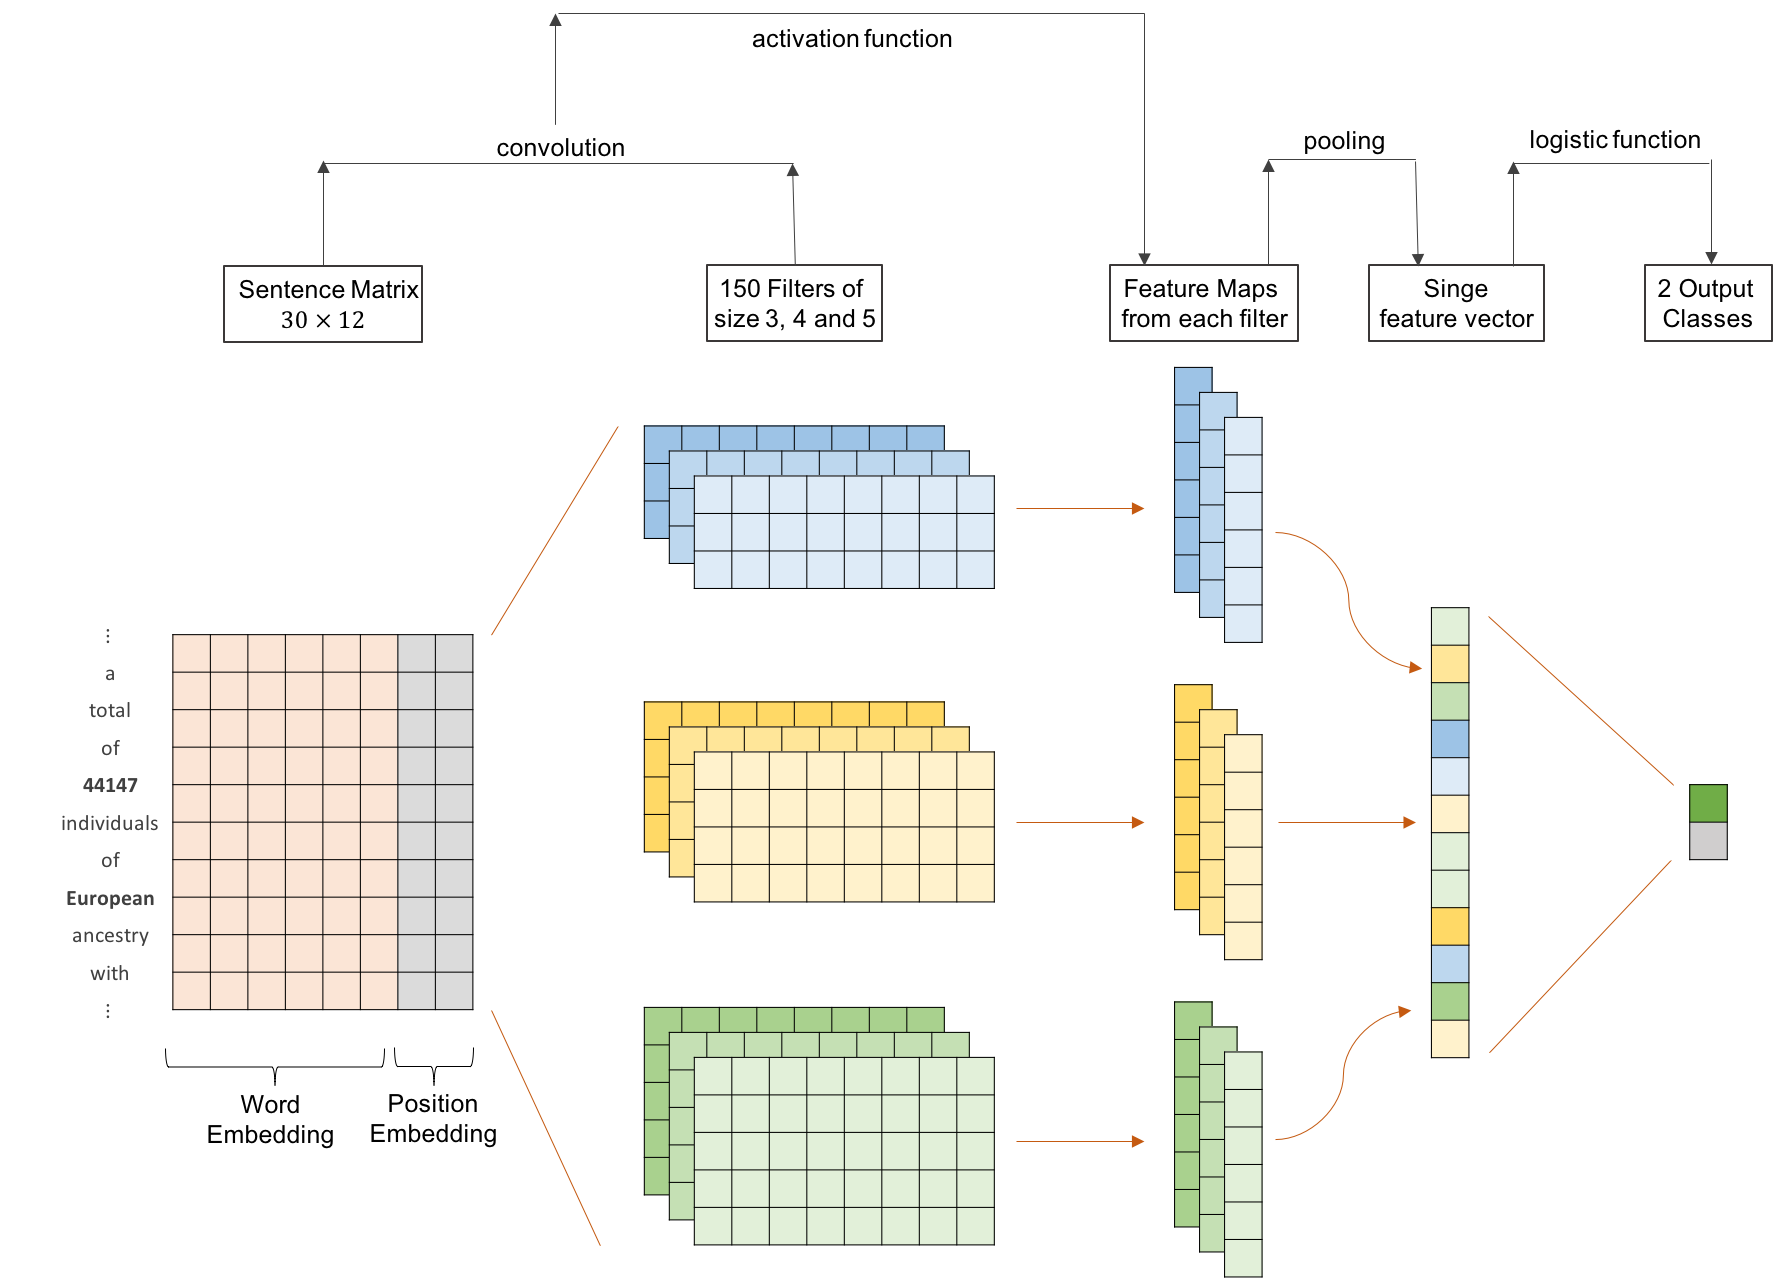
\includegraphics[width=\linewidth]{Images/Complete-CNN-Framework.png}
    \caption{Updated architecture of our Convolutional Neural Network with a combination of multiple filter region sizes and illustration of different stages of processing in the overall model.}
    \label{figure:complete-cnn-framework}
\end{figure}